\documentclass{amsart}
\usepackage{graphicx,amsfonts,amsthm,amsmath,amssymb,enumerate,enumitem,xcolor,commath,hyperref} % Required for inserting images
\usepackage{geometry}[margin=1in]
\usepackage{biblatex}[sorting=none]

\title{An Introduction to Computational Stochastic PDEs\\ Exercises: Chapter 1}
\author{Chris DuPre }
\date{April 2024}

\theoremstyle{plain}
\newtheorem{thm}{Theorem}[section]
\newtheorem{lem}[thm]{Lemma}
\newtheorem{prop}[thm]{Proposition}
\newtheorem*{cor}{Corollary}

\theoremstyle{definition}
\newtheorem{defn}{Definition}[section]
\newtheorem{conj}{Conjecture}[section]
\newtheorem{exmp}{Example}[section]
\newtheorem{exer}{Exercise}[section]

\newcommand{\R}{\mathbb{R}}
\newcommand{\C}{\mathbb{C}}
\newcommand{\Z}{\mathbb{Z}}
\newcommand{\Q}{\mathbb{Q}}
\newcommand{\N}{\mathbb{N}}
\newcommand{\Hil}{\mathcal{H}}
\newcommand{\E}{\mathcal{E}}

\newcommand{\tcr}[1]{\textcolor{red}{#1}}

\bibliography{Ref}

\begin{document}

\maketitle
\setcounter{section}{1}
\begin{exer}
For a bounded domain $D$, prove that $C\left(\overline{D}\right)$ is complete with respect to the supremum
norm $\|u\|_{\infty} = \sup_{x \in D} \abs{u(x)}$. By constructing a suitable Cauchy sequence, show that
$C\left(\overline{D}\right)$ is not complete with respect to the $L^{2}(D)$ norm. 
\end{exer}
\begin{proof}
    First, note that $\overline{D}$ is bounded as $D$ is bounded. Thus by Heine-Borel, $\overline{D}$ is compact. As continuous functions achieve their supremeum on compact sets, each $f_k$ is bounded. Define $M_n := \sup_{y\in \overline{D}} f(y)$. We first claim that $f_k$ as a sequence is uniformly bounded. To see this, note that as $f_k$ is Cauchy, there exists an $N$ such that for all $m,l\geq N$ we have that $\|f_m-f_l\|_{\infty} < 1.$ We thus have that $\sup_{y\in \overline{D}} \abs{f_l(y)} \leq M_N + 1.$ We thus have that $\sup_{k\in \N, x\in \overline{D}}\abs{f_k(x)} \leq \max\left\{\{M_k\}_{k=1}^{N}\right\}+1.$
    \par 
    As these are uniformly bounded, in particular for every $y\in \overline{D}$, we have that $f_k(y)$ is bounded and Cauchy. As $\R$ is complete, it must converge. For every $x\in \R$, define
    $$f(x) = \lim_{k\to \infty} f_k(x).$$
    We claim that $\lim_{k\to \infty} \sup_{y\in D} \abs{f_k(y)-f(y)} = 0$, (we do not use the norm as a-priori we do not know this function is continuous). As $\abs{\cdot}$ and subtraction are continuous, it is clear that for every $y \in \overline{D}$ that
    $$\abs{f_{k}(y)-f(y)} \leq\lim_{m\to \infty}\abs{f_{k}(y)-f_{m}(y)} \leq \limsup_{m\to \infty} \|f_k -f_m\|_{\infty}.$$
    As the right hand side is independent of $y$, we may take the supremum over the right hand side. For all $\varepsilon > 0$, there exists an $N$ such that the right hand side is less than $\varepsilon$ if $k=N$. As $\varepsilon$ is arbitrary, it is clear that 
    $$lim_{k\to \infty} \sup_{y\in D} \abs{f_k(y)-f(y)} = 0.$$
    \par We now claim that $f$ is continuous. To see this, note
    $$\abs{f(x)-f(y)}\leq \abs{f(x)-f_k(x)}+\abs{f_k(x)-f_k(y)}+\abs{f_k(y)-f(y)}.$$
    By the previous statement, there exists a $k$ such that the first and last terms are less than $\varepsilon/3$ for all $x,y\in\overline{D}.$ As $f_k$ is then continuous, there exists $\delta > 0$ such that if the distance between $x,y$ is less than $\delta$ we have that the middle term is less than $\varepsilon/3$. Thus $f$ is continuous.
    \par As a counter example for $L^2$, consider
    $$f_k(x) = \begin{cases}
        0 & -2\leq x \leq -1-\frac{1}{k}\\
        \frac{k(x+1)+1}{2}& \abs{x+1}\leq \frac{1}{k}\\
        1 & \abs{x}\leq 1-\frac{1}{k}\\
        \frac{k(1-x)+1}{2}& \abs{x-1}\leq \frac{1}{k}\\
        0 & 1+\frac{1}{k}\leq x\leq 2
    \end{cases}$$
    \begin{figure}[h!]
        \centering
        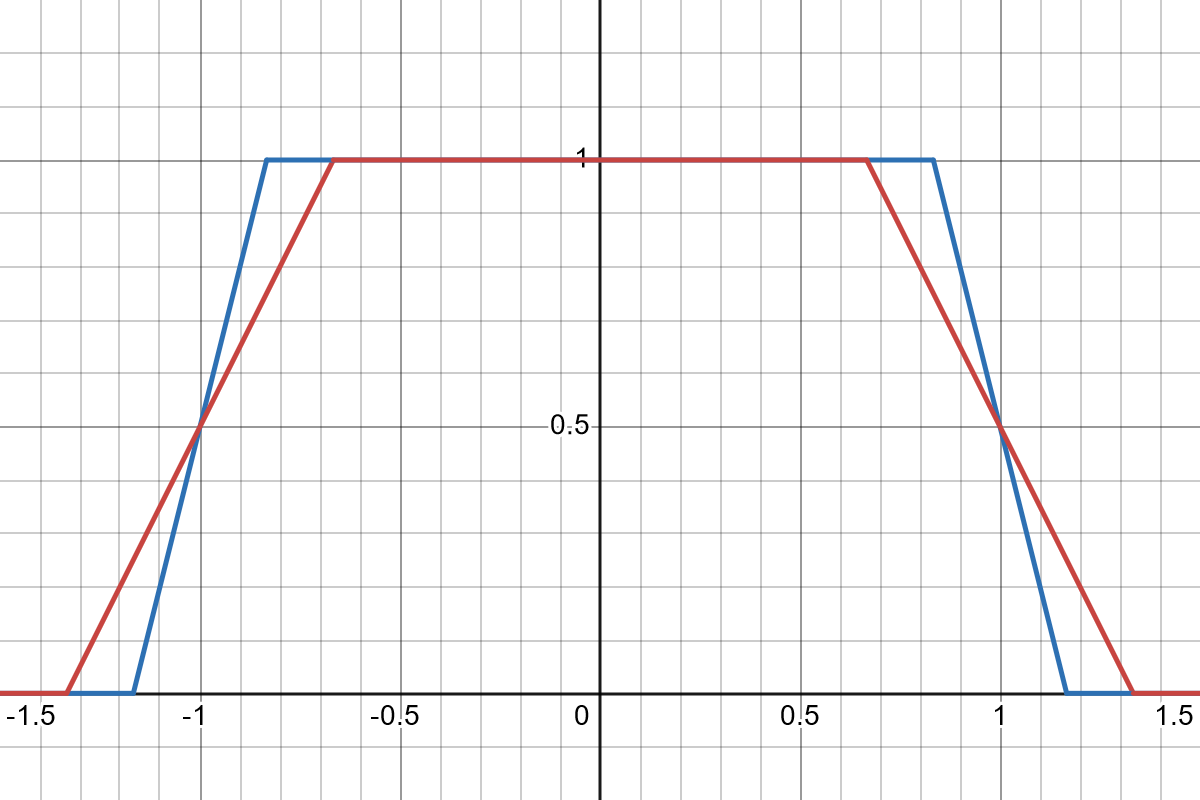
\includegraphics[width=0.5\linewidth]{Chapter 1/Photos/Problem1Counter.png}
        \caption{Depiction of counter example family. Red is $k=3$. Blue is $k=7$.}
        \label{fig:Problem_1_counter}
    \end{figure}
    This family is clearly continuous on $[-2,2].$ It is also clearly Cauchy, as in particular
    $$\|f_k - f_m\|_{L^2} \leq \frac{2}{\min_{m,k}}.$$
    However, this sequence converges to $\mathbf{1}_{[-1,1]}$ which is not continuous and therefore not in the space. Thus we have a Cauchy sequence which does not converge and the space is not complete
\end{proof}

\begin{exer}
    Let $\left(X,\mathcal{F},\mu \right)$ be a complete measure space, $Y$ be a Banach space, and $f : X \to Y$ a measurable function. Show that $f = g$ a.s. implies that g is measurable. Give an example to show that the completeness assumption on the measure space is necessary.
\end{exer}
\begin{proof}
Note that $f= g$ a.s. implies that there exists a measurable null set $N$ such that $f=g$ on $N^C$. Let $B$ be measurable and consider $g^{-1}(B).$ Then clearly $g^{-1}(B) = g^{-1}(B)\cap N \cup g^{-1}(B) \cap N^C = g^{-1}(B)\cap N \cup f^{-1}(B) \cap N^C.$ By completeness, $g^{-1}(B)\cap N$ is measurable. Thus $g^{-1}(B)$ is a finite union of measureable sets and is thus measureable. 
\par To see that completeness is neccesary. Consider $X = \{1,2,3\}, \mathcal{F} = \{\empty,\{1\},\{2,3\},\{1,2,3\}\}$ with $\mu\left(\{1\}\right) = 1, \mu\left(\{2\}\right)=\mu\left(\{3\}\right).$ Let $f$ be defined as $f(1) = f(2) = 0, f(3) = 0$ and $g(1)=g(3) = 1, g(2) = 0$. Note that $f = g$ a.s. with $N = \{2,3\}$ and $f$ is measureable but $g$ is not.  
\end{proof}

$$\int_{X} \|u(x)\|_{Y} dx < \infty.$$
\begin{exer}
   Using Definition 1.2.1 in \cite{lord2014introduction}, prove that if $u:X\to Y$ is integrable then 
        $$\int_{X} \|u(x)\|_{Y} dx < \infty.$$
\end{exer}
\begin{proof}
    Note that 
    \begin{align*}
        \int_{X} \|u(x)\|_{Y} dx &\leq \int_{X} \|u(x)-u_k(x)\|_{Y} dx + \int_{X} \|u_k(x)\|_{Y} dx \\
        & = \int_{X} \lim_{m\to \infty} \|u_m(x)-u_k(x)\|_{Y} dx + \int_{X} \|u_k(x)\|_{Y} dx \\
        & \leq \liminf_{m}\int_{X} \|u_m(x)-u_k(x)\|_{Y} dx+ \int_{X} \|u_k(x)\|_{Y} dx.
    \end{align*}
    The last inequality follows by Fatou's lemma. 
    For $k$ sufficiently large , the first term is bounded by $1$ by Definition 1.2.1. By the definition of simple functions, the second is also bounded. Thus the term on the left is bounded as well.
\end{proof}

\begin{exer}
\tcr{Newline}
    \begin{enumerate}[label=\alph*.]
        \item If $u:\R\to\R$ is measurable, define simple functions $u_n$ such that $u_n(x) \to u(x)$ for all $x\in\R.$
        \item If $G\in C\left(\R\times \R\right)$, define simple functions of the form
        $$\sum_{j,k=1}^{N} G(x_j,x_k)\mathbf{1}_{\mathcal{F}_j}\mathbf{1}_{\mathcal{F}_k}$$
        for $x_j\in\R, F_j \in \mathcal{B}\left(\R\right)$, such that $G_j\to G$ point-wise as $N\to \infty.$
    \end{enumerate}
\end{exer}
\begin{proof}\tcr{Somehow}
    \begin{enumerate}[label=\alph*.]
        \item Define $\mathcal{F}_{j}^{n} = u^{-1}\left(\left[\frac{j}{n},\frac{j+1}{n}\right)\right)\cap\left[-n,n\right], -n^2 \leq j \leq n^2$ and define:
        $$u_n(x) = \sum_{j=-n^2}^{n^2} \frac{j}{n}\mathbf{1}_{\mathcal{F}_{j}^{n}}.$$
        It is clear this function is simple as each set is clearly measurable and $\mu\left(\mathcal{F}_j^n\right)\leq 2n$. Consider $x\in \R$. Then for $n\geq \lceil \abs{x}\rceil$, we have that $\abs{u(x)-u_{n}(x)}\leq \frac{1}{n}$ and thus it converges point-wise.
        \item Let $F_j^n = \left[\frac{j}{n},\frac{j+1}{n}\right), -n^2 \leq j \leq n^2$ and define 
        $$G_n(x,y) = \sum_{j=-n^2}^{n^2}\sum_{k=-n^2}^{n^2} G\left(\frac{j+1/2}{n},\frac{k+1/2}{n}\right)\mathbf{1}_{F_j^n}(x)\mathbf{1}_{F_k^n}(y).$$
        To see point-wise convergence, fix $(x,y) \in \R\times\R.$ As $G$ is continuous, for every $\varepsilon>0$ there exists an $N$ large enough such that if $(x_1,y_1)$ and $(x_2,y_2)$ are less than $\frac{1}{\sqrt{2}N}$ apart then $\abs{G(x_1,y_1)-G(x_2,y_2)}\leq \varepsilon$. For each such $\varepsilon$, pick $n \geq \max\{\lceil \abs{x}\rceil, \lceil \abs{y} \rceil, N\}.$ We then claim that $\abs{G_n(x,y)-G(x,y)}\leq \varepsilon.$ This is because every point is shifted to another point at most $\frac{1}{\sqrt{2}N}$ away, which is chose so that the difference is less than $\varepsilon.$
    \end{enumerate}
\end{proof}

\begin{exer}
    Give an example of a Lebesgue integrable function $u : R \to R$ that is not Riemann integrable.
\end{exer}
\begin{proof}
Let $f$ be defined as 
$$f(x) = \begin{cases}
    1 & x\in \Q\\
    0& \text{else}.
\end{cases}$$
It is clear that $f$ is Lebesgue integrable and that in fact $\int \abs{f}dx = 0.$ However, we claim $f$ is not integrable. This is because the function is not of finite variation. This can be seen by taking the sequence of partitions $\pi_n=\cup_{j=0}^{n-1} \left[\frac{j}{n}, \frac{j+\pi/4}{n}\right) \cup \left[\frac{j+\pi/4}{n},\frac{j+1}{n}\right)$. The variation at each level in this partition is clearly $2n$ and is thus unbounded. 
\end{proof}

\begin{exer}
    By introducing a measure on $\Z$, show that 
    $$\lim_{n\to \infty} \sum_{j\in \Z} u_{n,j} \to \sum_{j\in \Z} u_{j}$$
    if $\lim_{n\to\infty} u_{n,j} = u_{j}$ and such that $\abs{u_{n,j}} \leq U_{j}$ for some $U_j$ such that $\sum_{j\in\Z} U_j < \infty.$
\end{exer}
\begin{proof}
    Take the counting measure, where $c(A) = \abs{A}$ where $A\subset \Z$ and $\abs{A}$ is the sets cardinality. The result now follows by Lebesgue dominated convergence theorem. 
\end{proof}

\begin{exer}
    Evaluate
    $$\int_{0}^{b}\int_{0}^a f(x,y) dx dy , \int_{0}^{a}\int_{0}^{b} f(x,y) dy dx.$$
    Where 
    $$f(x,y) = \begin{cases}
        \frac{xy\left(y^2-x^2\right)}{\left(x^2+y^2\right)^3}  & (x,y) \neq (0,0)\\
        0 & (x,y) = (0,0).
    \end{cases}$$
    Why does Fubini's theorem \textit{not} apply?
\end{exer}
\begin{proof}
    For the computations, we have
    \begin{align*}
        \int_{0}^{b}\int_{0}^a f(x,y) dx dy &= \int_{0}^b \left[\frac{1}{2}\frac{x^2y}{\left(x^2+y^2\right)^2}\right]_{x=0}^{x=a} dy\\
        &= \frac{1}{2}\int_{0}^b \frac{a^2 y}{\left(a^2+y^2\right)^2} dy\\
        &= \frac{-1}{4}\left[\frac{a^2}{a^2+y^2}\right]_{y=0}^{y=b}\\
        &= \frac{1}{4}\left[1-\frac{a^2}{a^2+b^2}\right]=\frac{b^2}{4\left(a^2+b^2\right)}\\
        \int_{0}^{a}\int_{0}^b f(x,y) dy dx &= \int_{0}^b \left[\frac{-1}{2}\frac{xy^2}{\left(x^2+y^2\right)^2}\right]_{y=0}^{y=b} dx\\
        &= \frac{-1}{2}\int_{0}^a \frac{b^2 x}{\left(b^2+x^2\right)^2} dx\\
        &= \frac{-1}{4}\left[\frac{b^2}{b^2+x^2}\right]_{x=0}^{x=a}\\
        &= \frac{1}{4}\left[1-\frac{b^2}{a^2+b^2}\right]=\frac{a^2}{4\left(a^2+b^2\right)}.
    \end{align*}
    The reason Fubini's does not imply is it is not absolutely integrable. In fact, in polar coordinates the function takes the form $f(r,\theta) = \frac{\sin(4\theta)}{4r^2}.$ Therefore, any cone about $\theta=\pi/8+n*\pi/4, n\in\Z$ will show exactly this problem.
\end{proof}

\begin{exer}
    Using Fubini's theorem, prove that 
    $$\frac{1}{\sqrt{2\pi}}\int_{-\infty}^{\infty} e^{-\frac{x^2}{2}}dx = 1.$$
\end{exer}
\begin{proof}
Formally multiplying this integral with itself gives 
$$\frac{1}{2\pi}\int_{\R^2} e^{-\frac{x^2+y^2}{2}} dx dy$$.
As this function is non negative, we can show that if it is integrable, it is absolutely integrable. Transferring to polar coordinates gives
$$\frac{1}{2\pi}\int_{r=0}^{\infty}\int_{\theta=0}^{2\pi} e^{-\frac{r^2}{2}} r dr d\theta = 1.$$
Thus the function is integrable and its square is 1. As the function is non-negative, the integral must be 1.   
\end{proof}

\begin{exer}
    For $f\in C^1\left( [0,1] \right)$ and $p\geq 1$, prove that
    $$\left(\int_0^1 \abs{f(x)} dx\right)^p \leq \int_0^1 \abs{f(x)}^p dx$$
    This is a version of Jensen's inequality. For $a<b$, show that $L^q (a,b)\subset L^p(a,b)$ for $1\laq p \leq q.$
\end{exer}
\begin{proof}
By H\"older's inequality
$$\int_0^1 \abs{f(x)}\times 1 dx \leq \left(\int_0^1 \abs{f(x)}^p\right)^{1/p} \left( \int_0^1 dx\right)^{1/q} = \left(\int_0^1 \abs{f(x)}^p\right)^{1/p}.$$ 
Raise both sides to the $p$ power to obtain the desired inequality. Let $1\leq p\leq q$. Let $r = \frac{q}{p}.$ Applying the above procedure with $r$ gives
$$\int_a^b \abs{f(x)}^p\times 1 dx \leq \left(\int_a^b \abs{f(x)}^q\right)^{1/r} \left( \int_a^b dx\right)^{1-1/r} = \left(\int_0^1 \abs{f(x)}^p\right)^{p/q} \left(b-a\right)^{\frac{q-p}{q}}.$$
Raising both side to $1/p$ bounds the left hand side by a constant multiple of the right hand side. Thus if $f\in L^q$, $f\in L^p$ or $L^q([a,b]) \subset L^p([a,b]).$
\end{proof}

\begin{exer}
    On a real Hilbert space $H$, prove the Cauchy–Schwarz inequality $\abs{\langle u, v\rangle}\leq \|u\|\|v\|$ for $u,v\in H.$
\end{exer}
\begin{proof}
If both $u = 0$ and $v= 0$, the statment is trivial. Assume without loss $v \neq 0$. Consider $f(\alpha) = \|u+\alpha v\|^2.$ Taking the derivative with respect to $\alpha$ gives $\frac{df}{d\alpha} = -2\langle u,v\rangle + 2\alpha \|v\|_{2}^{2}.$ Seeking an critical point gives $\alpha = \frac{\langle u,v\rangle}{\|v\|^2}.$ Evaluating at this critical point gives 
$$0\leq \|u+\alpha v\|^2 = \|u\|^2 - 2\frac{\langle u,v\rangle^2}{\|v\|^2}+\frac{\langle u,v\rangle^2}{\|v\|^2} = \|u\|^2 - \frac{\langle u,v\rangle^2}{\|v\|^2}.$$
Rearranging and taking the square root of both sides gives the Cauchy-Schwarz inequality.
\end{proof}

\begin{exer}
    Prove that $(1.12)$ is the weak derivative of $(1.11)$  (by showing that $(1.13)$ holds) (Equations on p. 12 of \cite{lord2014introduction}) and that $\mathcal{D}u$ does not have a weak derivative in the set of measurable functions $u:\R\to\R.$
\end{exer}
\begin{proof}
Assume by density that $\phi \in C^\infty_c(\R).$
    \begin{align*}
        \int_\R \mathcal{D}u(x) \phi(x) dx &= \int_{0}^\infty \phi(x) dx \\
        &= -\int_{0}^\infty x\phi'(x)dx = -\int_{\R} u(x)\phi'(x) dx. 
    \end{align*}
\end{proof}

\begin{exer}
    \begin{enumerate}[label=\alph*.]
        \item Let $u(r) = \log\left(\abs{\log(r)}\right)$ for $r> 0$. Sketch a graph of $u(r)$ and $u'(r).$ Show that $u\in L^2\left(\left[0,\frac{1}{2}\right]\right)$ but $u\not \in C\left(\left[0,\frac{1}{2}\right]\right)$ and $u' \not \in L^2\left(\left[0,\frac{1}{2}\right]\right)$
        \item
    \end{enumerate}
\end{exer}
\begin{proof}
    \begin{enumerate}[label=\alph*.]
        \item By direct computation $u'(r) = \frac{1}{r\log(r)}$. A sketch of two graphs is shown below.
        \begin{figure}[h!]
            \centering
            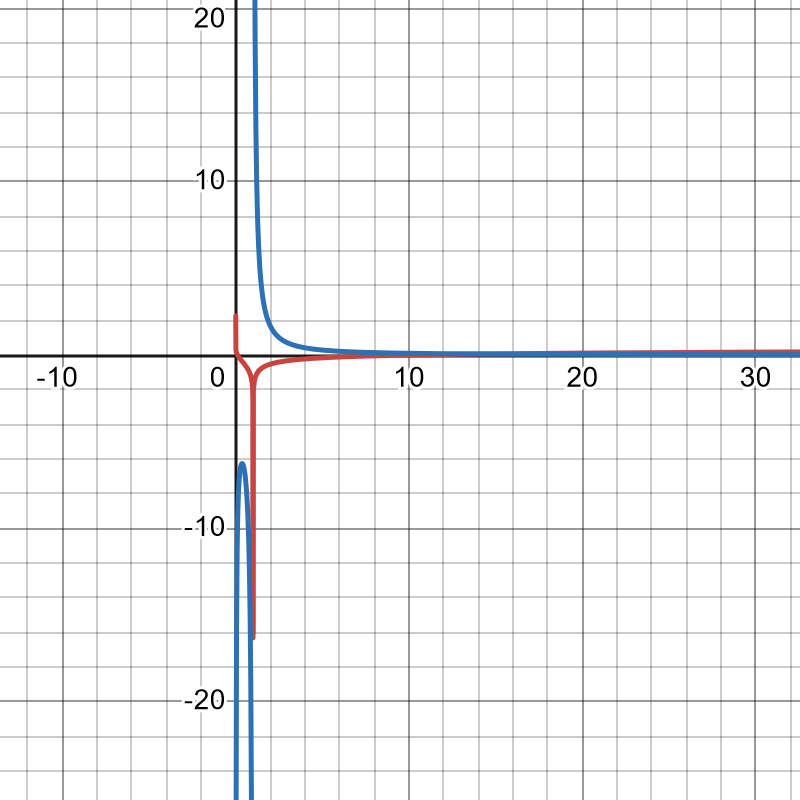
\includegraphics[width=0.5\linewidth]{Chapter 1/Photos/Problem12A.png}
            \caption{Sketch of \textcolor{red}{$u(r)$} and \textcolor{blue}{$u'(r)$}.}
            \label{fig:12a}
        \end{figure}
        To see $u\in L^2([0,1/2])$ we can compute:
        $$\int_0^{1/2} \log\left(-\log x\right) dx = \int_{2}^{\infty} \frac{\log\left(\log u\right)^2}{u^{1/2}}\frac{1}{u^{3/2}}du.$$ Notice that for all $x\geq 0$ we have that $\log(x) < x$ and that $\log(x)$ is increasing so $\log(\log(x))^2 \leq \log(x)^2.$ 
        Further, we have that $x^{1/2} > \log(x)^2$ for all $x\geq 1$. Thus we have that
        \begin{align*}
            \int_0^{1/2} \log\left(-\log x\right) dx &= \int_{2}^{\infty} \frac{\log\left(\log u\right)}{u^{1/2}}\frac{1}{u^{3/2}}du\\
            &\leq \int_2^\infty \frac{1}{u^{3/2}} du = \left[\frac{-2}{u^{1/2}}\right]_{u=2}^{u=\infty} =  \frac{1}{\sqrt{2}} < \infty.
        \end{align*}
        Thus $u\in L^2([0,1/2]).$ u does not admit a continuous extension as in particular $\lim_{n\to\infty} \abs{u\left(\frac{1}{n}\right)} = \infty$ so $u(0)$ cannot be defined. $u'(r)\not \in L^2([0,1/2])$ as by direct computation:
        $$\int_{0}^{1/2} \frac{1}{r^2\log(r)^2} dr \geq \int_{0}^{1/2} \frac{1}{r\log(r)^2} \frac{1}{r}dr.$$
        Notice that for all $x\leq 1$ we have that
        $\frac{1}{x\log(x)^2} \geq 1.$ Thus we have that 
        \begin{align*}
            \int_{0}^{1/2} \frac{1}{r^2\log(r)^2} dr &= \int_{0}^{1/2} \frac{1}{r\log(r)^2} \frac{1}{r}dr\\
            &\geq \int_{0}^{1/2}  \frac{1}{r}dr.
        \end{align*}
        But the last integral diverges. Therefore $u'\not \in L^2([0,1/2])$
        \item
    \end{enumerate}
\end{proof}

\printbibliography
\end{document}
